\documentclass{article}

\usepackage{lipsum}
\usepackage[left=1in, right=1in, top=1in, bottom=1in, includefoot]{geometry}
\usepackage{amsmath,amssymb}
\usepackage{setspace}
\usepackage{indentfirst}
\usepackage{setspace}
\usepackage{blindtext}
\usepackage{titlesec}
\usepackage{slashed}
\usepackage{physics}
\usepackage{tensor}
\usepackage{array}
\usepackage[T1]{fontenc}
\usepackage[utf8]{inputenc}
\usepackage{xspace}
\newcommand{\Poincare}{Poincar\'e\xspace}
\newcommand{\Lubanski}{Luba\'nski\xspace}
\newcommand{\Kahler}{K$\ddot{\text{a}}$hler\xspace}
\usepackage[skip=10pt plus1pt, indent=2em]{parskip}
\usepackage{mathtools}
 \usepackage{graphicx}
 \usepackage{dsfont}
 \usepackage{float}
\usepackage{subfig}
\usepackage{siunitx}
 %\usepackage{hyperref}
 \graphicspath{ {./image/} }

\title{Cavendish Experiment}
\author{Eric Yang, \AE ther Zhou, Kien Le }
%
\date{February 2023}

\begin{document}

\maketitle

\begin{abstract}
    We report an experiment to determine the universal gravitational attraction constant $G$ by performing the Cavendish torsion balance. We inferred the $G$ values by obtaining measurements for the small masses' acceleration, as well as deflection from equilibrium position via rotating the positions of the large masses. Our data indicated that the measured $G = (4.39 \pm 0.86) \times 10^{-11}$ m$^3$ kg$^{-1}$ s$^{-2}$ values with the available PASCO equipment is significantly below the accepted value $G = 6.674 \times 10^{-11} $ m$^3$ kg$^{-1}$ s$^{-2}$ by $34\%$. Our $20\%$ statistical error cannot explain this deviation, so we propose potential systematic error due to lagging in data recording and residual oscillation. 

\end{abstract}



\section{Introduction}

\subsection{Background}

The Cavendish experiment is done by studying a gravitationally induced oscillation process. To be more specific, consider a horizontally placed pendulum with its center fixed and two small masses attached to its ends. One can create a torque on the pendulum by placing two large masses near the small masses, which induces an angular oscillation. Since gravity is the main external force, various parameters of the oscillation, such as period and amplitude, are necessarily functions of the gravitational constant. 
    
The main obstacle is the gravitational attraction on the masses due to the Earth. This force acts vertically on all test masses and significantly dominates over the gravitational attraction between any test masses. Thus, the entire device must be placed on a level surface. To further negate the gravity due to Earth, one can consider attaching the pendulum to a torsion ribbon and hanging the pendulum at a fixed position. Under this setup, one can put two large test masses on the two ends of a large swivel horizontally placed at the same height as the pendulum, rotate the swivel, and use the gravitational attraction between the small mass and the large mass to create a torque on the pendulum. This torque generates an oscillation on the pendulum, which is necessarily damped due to the torsion ribbon. Our main task is to study this oscillation and extract $G$ from various characteristic quantities of this motion. 
    


%Determination of a small physical constant like the gravitational constant $G$ is among the most important and yet simplest experiments one could do. 



\subsection{Theory}

When the hanging small masses ($m_2$) pendulum bob is gravitationally attracted to the external large masses ($m_1$), the forces acting on the small masses are:
\begin{align}
    F &= G \frac{m_1 m_2}{b^2} 
\end{align}
Where $b$ is the distance between the centers of the two masses. When the small masses in equilibrium are subjected to a change in the large masses' gravitational attraction's direction, the small masses will experience a new force:
\begin{align}
    m_2 a_0 = 2 F =  2 G \frac{m_1 m_2}{b^2}
\end{align}
Relating this expression to the equation for small masses linear displacement due to constant acceleration $\Delta s = a_0 t^2 / 2$ gives: 
\begin{align}
    a_0 = 2G\frac{m_1}{b^2} = \frac{2\Delta s}{t^2}
\end{align}
Relating $\Delta s$ to light spot displacement $\Delta S$, we have:
\begin{align}
    a_0 = 2G\frac{m_1}{b^2} = \frac{\Delta S d}{t^2 L}
\end{align}
Where $d$ is the distance between two small masses and $L$ the distance from the light spot on the screen to the mirror attached to the pendulum bob. 

\subsection{Experiment Summary}
Based on the theoretical description, we use the acceleration method to allow for a quick (Under 5 minutes) and relatively accurate measurement of the $G$ value, where we recorded the relative deflection $\Delta S$ as the pendulum bob moved away from an equilibrium position, and the acceleration was inferred by fitting $\Delta S$ versus $t^2$. 

\section{Experimental Methods}

\subsection{Description of Experimental Setup}
The rotation of the balance is converted to translation of light spot on the screen with a laser pointer. Hence, we are allowed to measure the small deviation of the balance in a relatively high precision. Figure~\ref{fig:set_up} shows some details about the setup. 
\begin{center}
    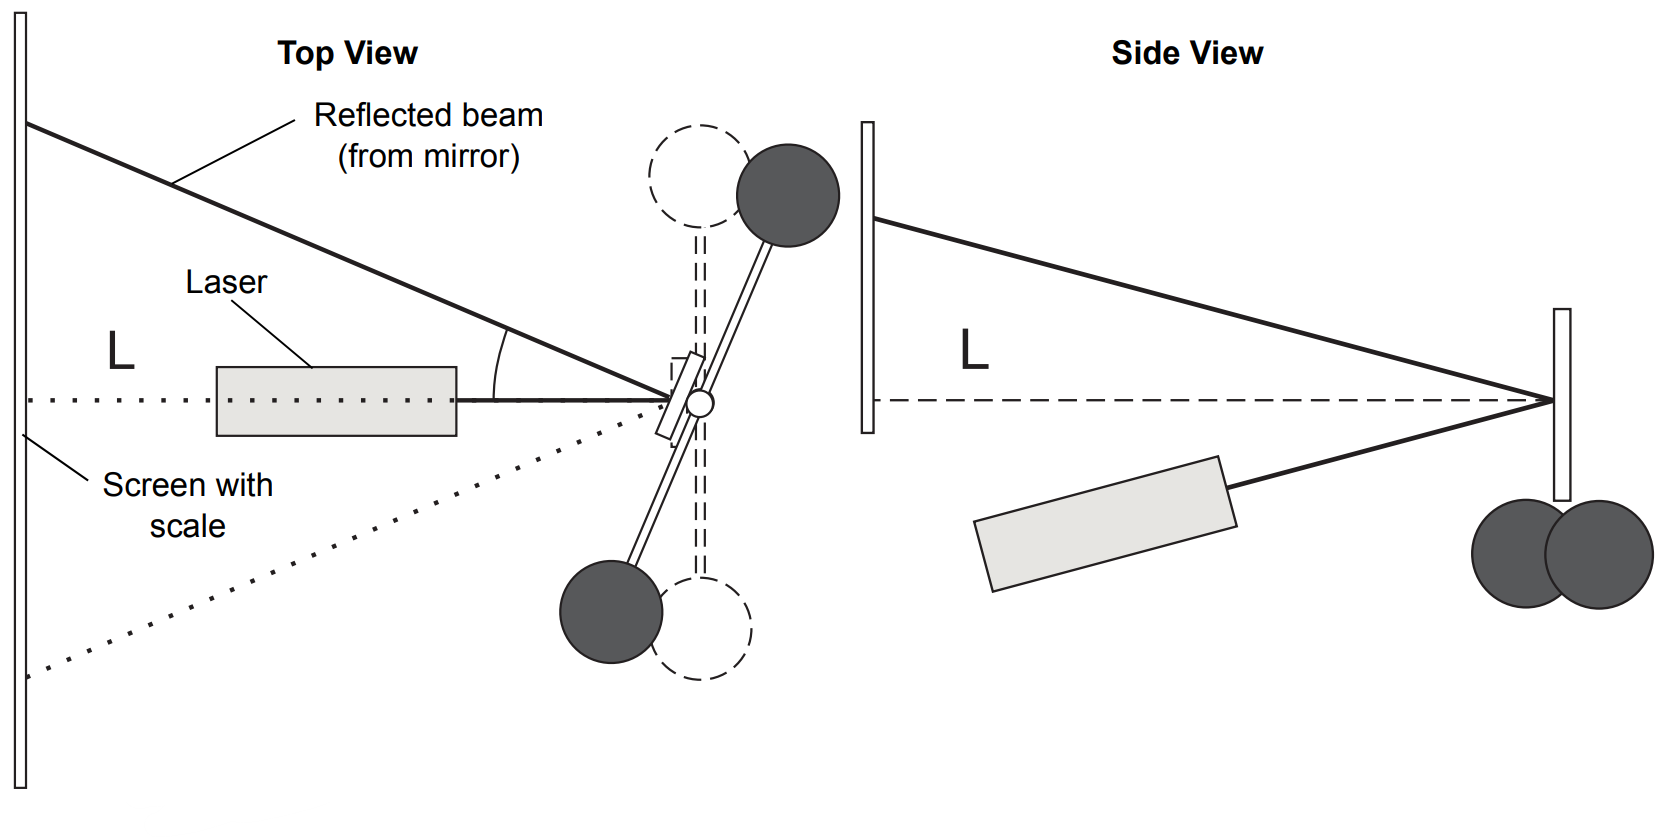
\includegraphics[width = 0.8\textwidth]{figures/setup_fig8.png}
    \captionof{figure}{Schematic for Cavendish torsion balance apparatus. }
    \label{fig:set_up}
\end{center}

Measuring $G$ by acceleration was performed in two steps. First, we needed to set up the experiment such that we found the equilibrium position when the large masses bob was placed in  $S_1$. To equilibrate the pendulum, we observed the light spot reflected from the mirror on the small masses pendulum for about two hours. When the oscillation's amplitudes had reduced to less than a tenth of the original amplitude (approximately 12 cm), we determined the approximate equilibrium position. Then, we turned the large masses to the $S_2$ position, and started recording videos of the acceleration process. 

\subsection{Relevant Parameters}
We report the relevant parameters for our analysis 
\begin{align*}
    d &= 50.0 \;\si{mm} \\
    b &= 42.2 \;\si{mm} \\
    m_1 &= 1500 \;\si{g} \pm 10 \;\si{g} \\
    m_2 &= 38.2 \;\si{g} \pm 0.2 \;\si{g}
\end{align*}

\subsection{Data Collection}

For the videos we recorded, we obtained positions of the laser spot by reading off where the laser spot was on the measure tape. As the spot moved very slowly, with a period of about 558s over an amplitude of less than 10 cm, we could obtain data for every 10s interval on the video. Since we recorded both the equilibrium calibration and acceleration videos, we wrote down the positions of the laser spot from both videos. These positions would then be plotted to infer equilibrium and acceleration needed for computing $G$. 

\section{Raw Data}

After calibrating the equipment, we quickly move the mass from position I to position II while record the motion of the laser dot on the screen by taking a 45-minute long video. The position of the laser dot is recorded every 10 second. Fig 1 shows a plot of the position of the laser dot against time. Over the 45 minute interval, the plot displays an obvious damped oscillation of the laser dot around some equilibrium position. Using this data, we can extract the equilibrium position by computing the midpoint between neighboring extrema. The average position between neighboring extrema and their time spans are recorded in table 1. The equilibrium position is $44.23$ $\pm$ $ 0.19$ cm. 

    To extract the gravitational constant, we focus on a short period of time shortly after the perturbation is introduced. This is because only in this region can we claim $a \sim \frac{\Delta S}{t^2}$ in (4) as a valid approximation. We choose to focus on the data of the first minute after the perturbation is introduced, which is shown in table 2. Using table 2, we made a plot of $\Delta S$ against $t^2$ to check the validity of the data, which is shown in fig 2. Since fig 2 apparently matches the linear relation $ \Delta S= (a_0 L/d) t^2$
    between $\Delta S$ and $t^2$, we can proceed to extract the gravitational constant with this data.

            

\begin{center}
    %\begin{table}
        \centering
        \begin{tabular}{|c |c |}
            \hline
        Time Intervals (s) & Middle Point between Extrema (cm) \\
\hline     \hline
            250-550 & 44.5\\
            \hline
            550-830 & 44.05\\
            \hline
            830 - 1090 &44.35\\
                            \hline
            1090 - 1300 &44.1\\
                            \hline
            1360 - 1640 & 44.35\\
                            \hline
            1640 - 1910 & 44.05 \\
                            \hline
            1910 - 2190 &44.4\\
                            \hline
            2190 - 2470 &44 \\
            \hline
             Average: 557.5 s & Average: 44.23 cm $\pm$ 0.19 cm\\
            \hline
            Statistical Error: 17.1 s   & Statistical Error: 0.19 cm\\
            \hline
        \end{tabular}
        \captionof{table}{Distance between neighboring extrema and their time span}
        \label{tab:my_label}
    %\end{table}
\end{center}



            

\begin{center}
        \centering
        \begin{tabular}{|c |c |}
            \hline
        Time Stamp Squared $t^2$:  (s$^2$) & Distance $\Delta S$ from the Equilibrium Position (m) \\
\hline     \hline
            100 & -0.058\\
            \hline
            400 & -0.058\\
            \hline
            900 & -0.055\\
             \hline
            1600 & -0.053 \\
            \hline
            2500 & -0.051 \\
            \hline
            3600 &  -0.047\\
            \hline
        \end{tabular}
        \captionof{table}{Distance between neighboring extrema and their time span}
        \label{tab:my_label}
\end{center}




\subsection{Plot}

\begin{center}
    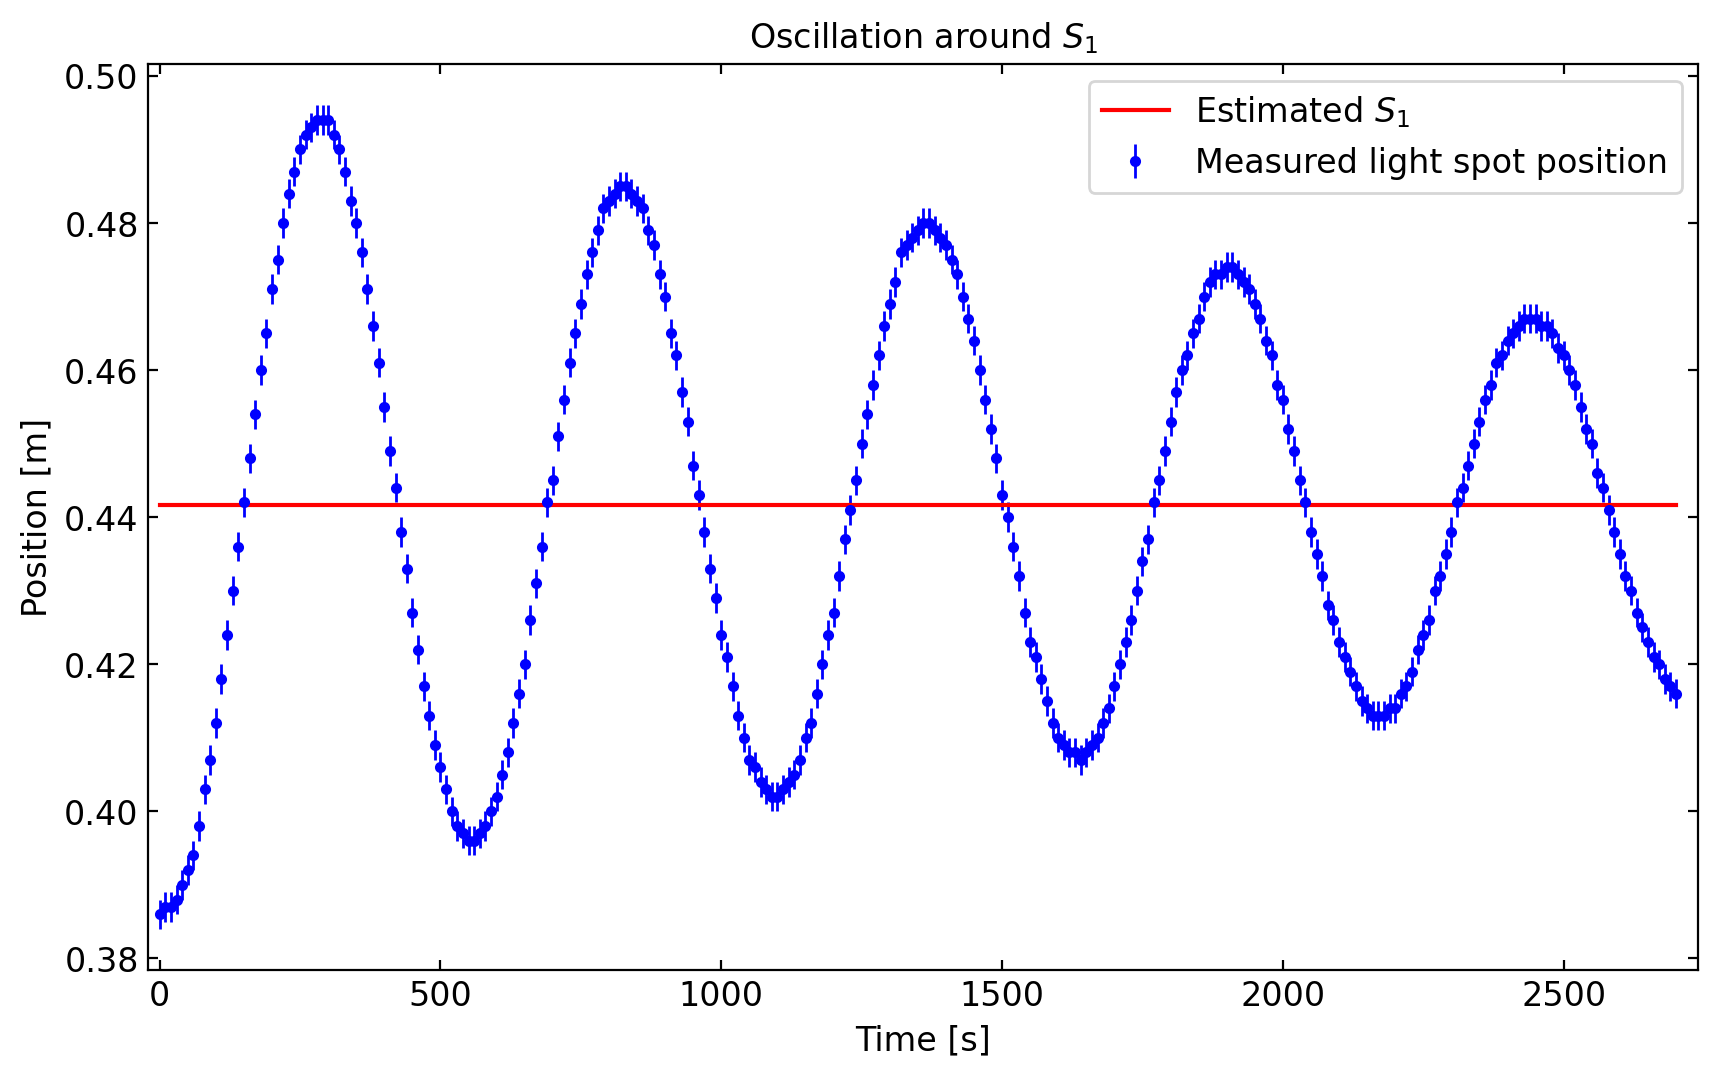
\includegraphics[width = 0.8\textwidth]{figures/Position 1.png}
    \captionof{figure}{Measuring light spot's oscillation about equilibrium position 1 ($S_1$), with $\pm 0.2$ cm errorbar representing uncertainty caused by the width of light spot. We took average of our data in time to estimate equilibrium position 1.}
    \label{fig:eq_s1}
\end{center}


\begin{center}
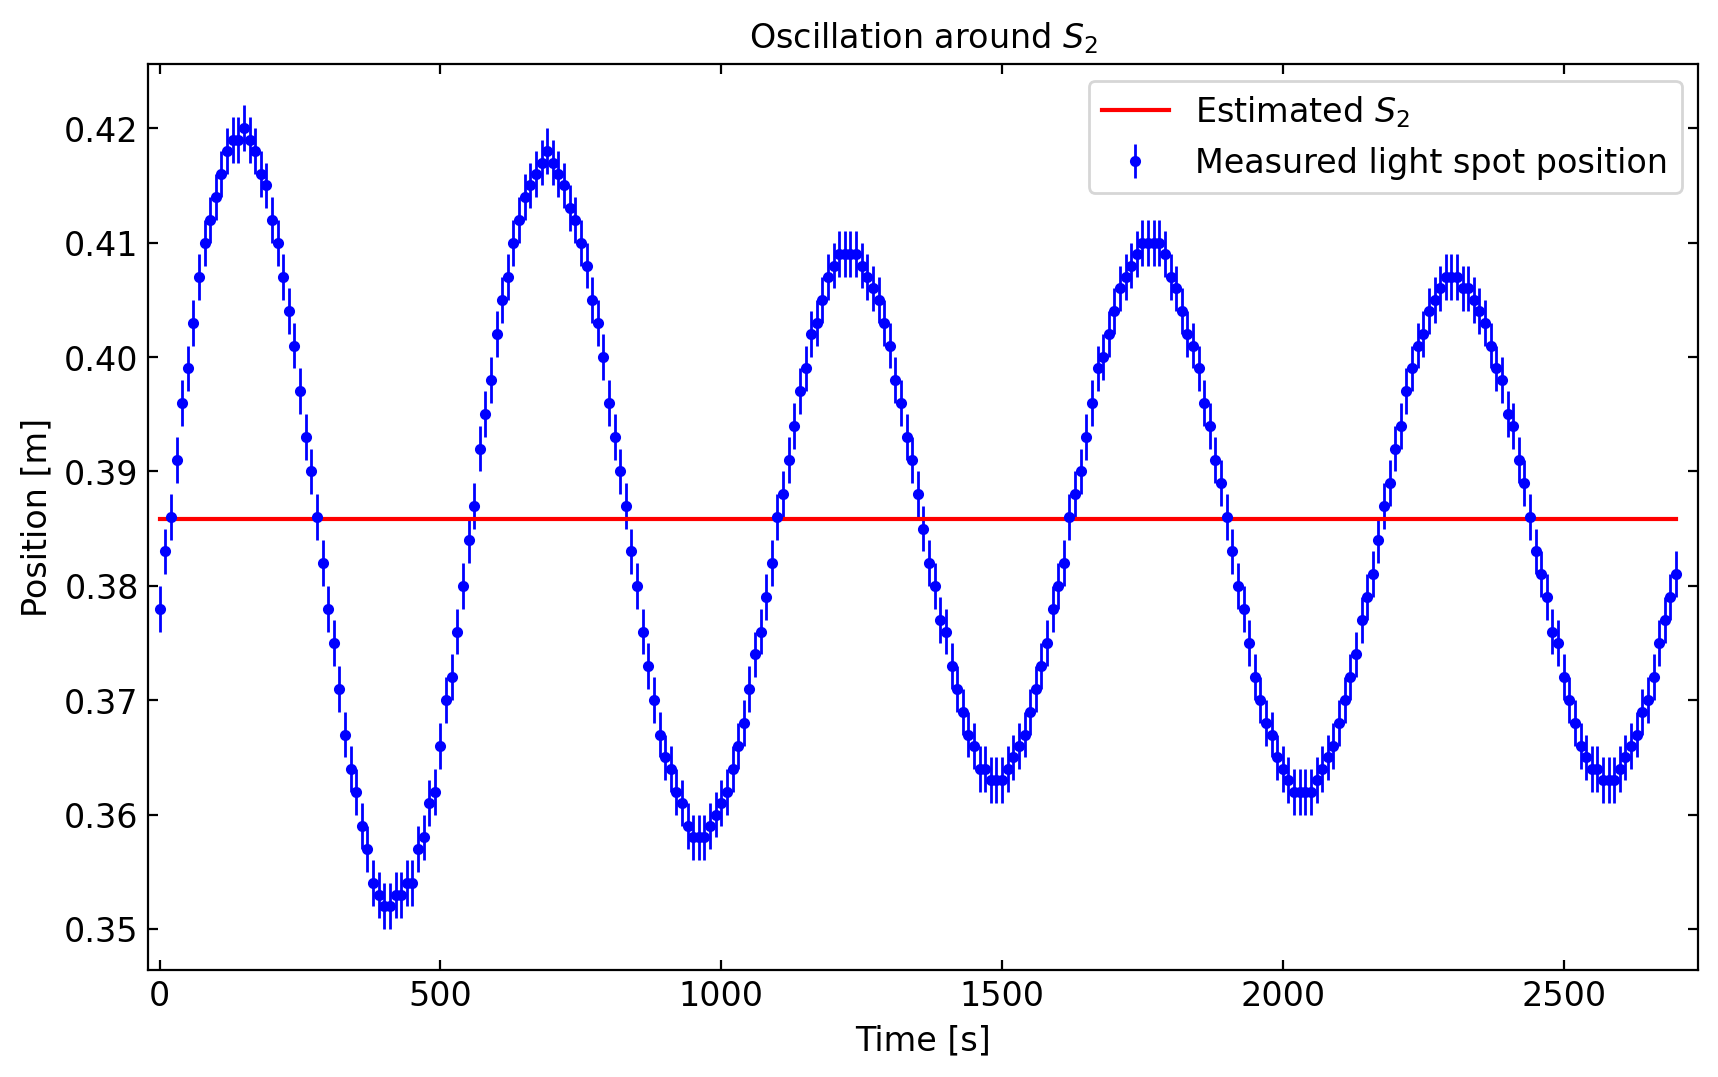
\includegraphics[width = 0.8\textwidth]{figures/Position 2.png}
\captionof{figure}{After we moved the large masses, we measured the light spot's oscillation about equilibrium position 2 ($S_2$), with $\pm 0.2$ cm errorbar representing uncertainty caused by the width of light spot. And we averaged our data in time to estimate equilibrium position 2.}
\label{fig:eq_s2}    
\end{center}


\subsection{Note on Plots}
The error bar for each data point comes from considering the width of the light spot, which was measured to be 0.2 cm on the ruler. The spot remained in the same width throughout the experiment, hence the uncertainty that we included stays within 0.2 cm. We also make a note on how in Figure~\ref{fig:eq_s1} the amplitude over time decayed consistently, but in Figure~\ref{fig:eq_s2} the amplitude decayed but stopped decaying in the interval between 1200 s to 1700 s


\section{Results}

\subsection{Data Analysis}

    According to (4), to extract the gravitational constant, we need to perform a linear fit of $\Delta S$ against $t^2$. The resulting slope is: 
        \begin{equation}
              \text{slope} = a_0 \cdot \frac{L}{d}
        \end{equation}
Using python scipy.curve\_fit, we manage to extracted the following slope (see Fig~\ref{fig:fit_a0}) $ 3.05 \times 10^{-6} \; \si{m/s^2}$. We take $d$ to be exact. $L$ gives the distance between the reflecting mirror in the Cavendish torsion device and the equilibrium position of the laser dot. We used Pythagorean's theorem in $\mathbb{R}^3$ and obtained $L = 217.4 \; \si{cm} \pm 0.05 \; \si{cm}$, where $0.05 \; \si{cm}$ is a systematic error given by one half of the smallest distance our ruler can measure. Plugging $d$ and $L$ into (5), we have:
    \begin{equation}
        a_0 = \text{slope} \cdot \frac{d}{L} = 3.05 \times 10^{-6} \; \si{m/s^2} \cdot \frac{0.05 \; \si{m}}{2.17 \; \si{m}} = 6.91 \times 10^{-8} \; \si{m/s^2}
    \end{equation}
Finally, plugging this result into the first half of (4), we find:
    \begin{equation}
        G = \frac{a_0 \cdot b^2}{2 m_1} = \frac{(6.91\cdot10^{-8}\; \si{m/s^2}) \cdot (0.042\; \si{m})^2}{2 \cdot 1.5\; \si{kg}} = 4.13 \times 10^{-11} \; \si{m^2.kg^{-1}.s^{-2}}
    \end{equation}
    
\begin{center}
    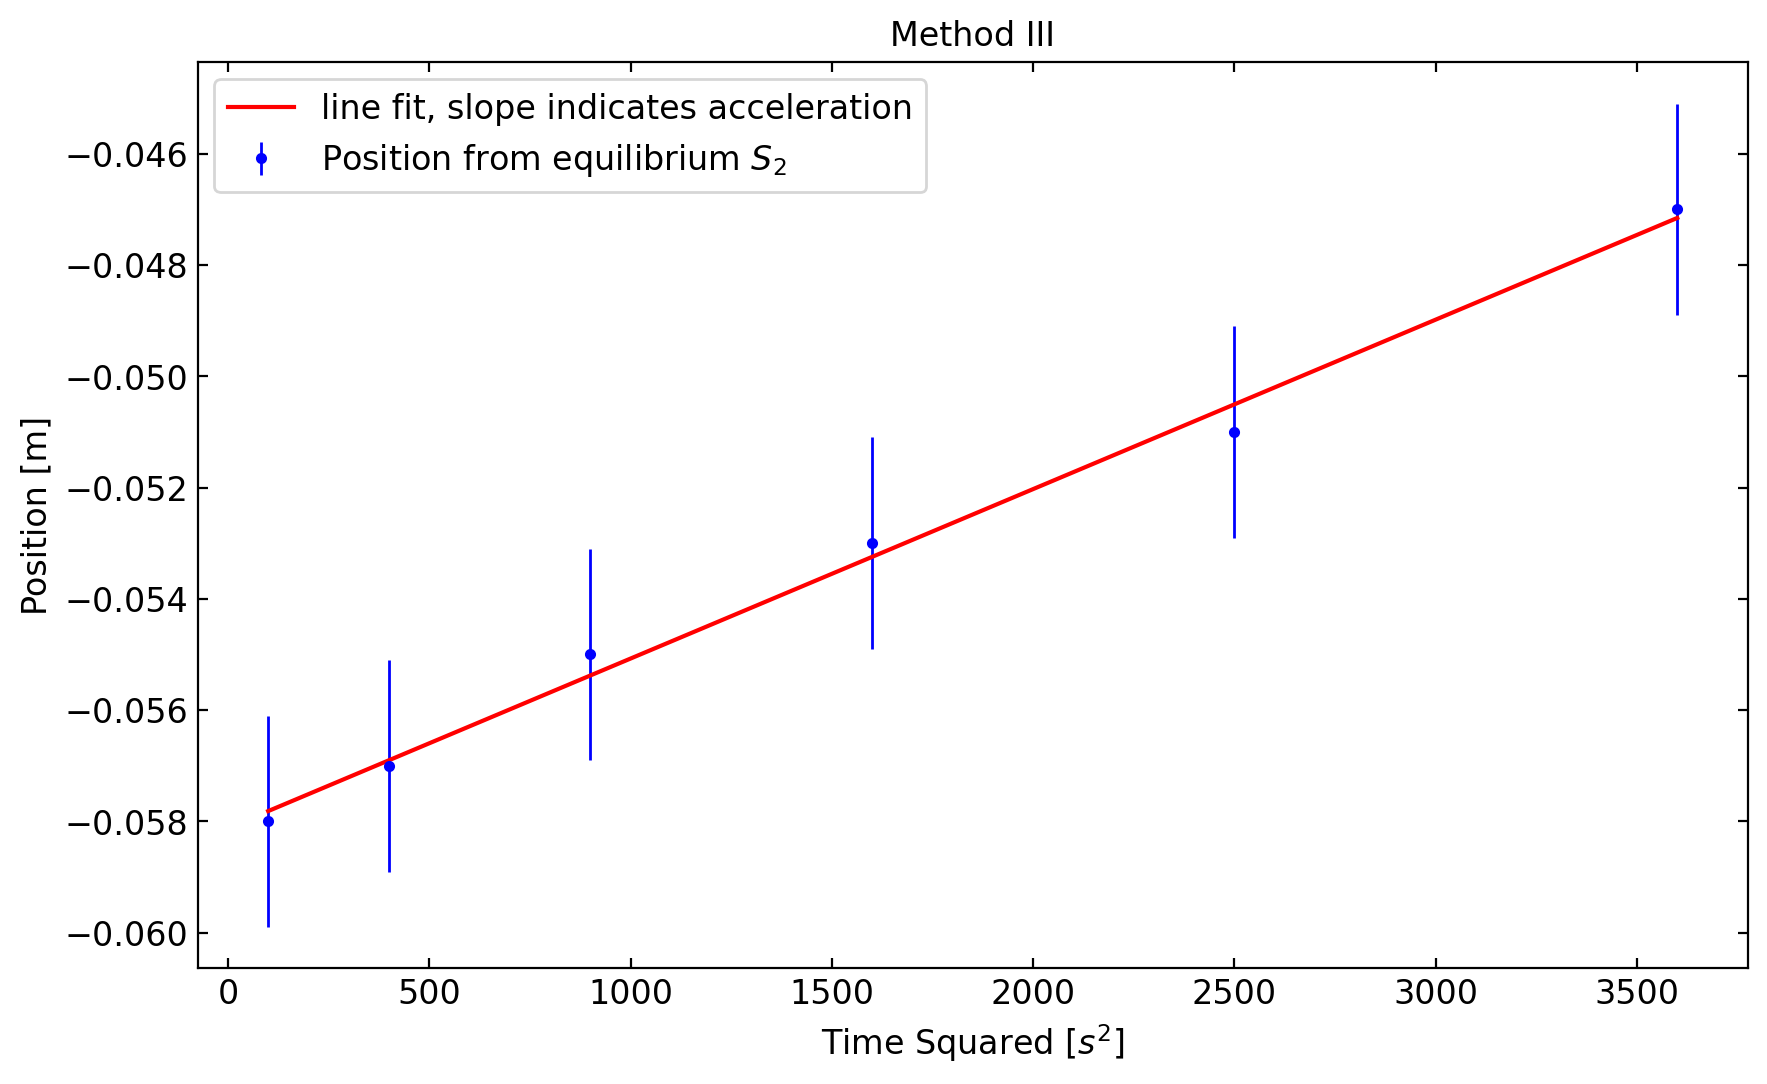
\includegraphics[width = 0.8\textwidth]{figures/Method III fit.png}
    \captionof{figure}{ \textbf{Analyzed Plot} - Around equilibrium position 2, we performed a line fit based on relative position from $S_2$ versus time squared. From this we can estimate acceleration (proportional to slope) and its uncertainty.}
    \label{fig:fit_a0}
\end{center}

\subsection{Error Analysis and Comments}
\subsubsection{Statistical Analysis}
In this subsection, we perform error propagation on our main measurement. For convenience, here we list all relevant formulas: 
		\begin{equation}
			G = b^2 \frac{a_0}{2m_1} \qq{and } \Delta S = \Delta s \Big(\frac{2L}{d}\Big) \qq{and}a_0 = \frac{2\Delta s}{t^2} = \frac{\Delta S }{t^2 } \cdot \frac{d}{L}
		\end{equation}
The measured quantities are the acceleration $a_0$ and $\Delta S$, and the standard error propagation formula is:
	\begin{equation}
		\delta G = \sqrt{\left(\pdv{G}{a_0} \right)^2 (\delta a_0)^2 + \left(\pdv{G}{m_1} \right)^2 (\delta m_1)^2 } 
	\end{equation}
 
However, it turns out we cannot use (8) for our error analysis. In this lab, we were only able to obtain one set of sensible data, so we only have one statistical uncertainty in determining the equilibrium position of the laser dot, which gives the statistical error for $\Delta S$. To see how (8) fails, we write the gravitational constant in the following convenient form:
	\begin{equation}
		G = \frac{b^2}{2m_1} \cdot \frac{d}{t^2 L} \Delta S
	\end{equation}
A short calculation yields:
	\begin{equation}
		\delta G = \frac{b^2}{2m_1} \cdot \frac{d}{t^2 L} \delta (\Delta S)
	\end{equation}
Since $d$ and $b$ appear as parameters of the Cavendish torsion device in the instruction manual, we take them to be exact. For convenience, we also take $L$ to be exact. Now the appearance of time dependence of $\delta G$ in (11) makes this analysis unreliable since we can't assume exact certainty in measuring position versus time. 

As an alternative, we consider a $\chi^2$ goodness-of-fit provided by the SciPy library in python, which naturally calculates the uncertainty of fitted parameters. We can use the scipy.curve$\_$fit to extract an uncertainty on the slope based on the covariant matrix returned from curve$\_$fit. The $\chi^2$ method gives the following standard deviation on the slope:
    \begin{equation}
        \delta (\text{slope}) = 6.35 \times 10^{-7} \;\si{m\cdot s^{-2}}
    \end{equation}
Using this error, we can perform error propagation on $G$
, which gives:
    \begin{equation}
       \delta G = \frac{b^2}{2m_1}\delta a_0 = \frac{b^2}{2m_1}\cdot \frac{d}{L}\cdot \delta (\text{slope}) = 8.6\times10^{-12} \;\si{m^2kg^{-1}s^{-2}}
    \end{equation}

\subsubsection{Systematic Error}
The experimental set up for Cavendish torsion balance is subjected to systematic error due to external gravitational attraction between the small masses and their farther large masses neighbors (not the immediate large masses). To account for this systematic error, we quantify the effect of this attraction on the overall gravitational force, which is described by the following factor:
\begin{align}
    \beta = \frac{b^3}{(b^2 + 4d^2)^{3/2}}
\end{align}
With this factor, we have the corrected $G_0$ to be:
\begin{align}
    G_0 &= \frac{G}{1 - \beta}
\end{align}
Given the values of $b$ and $d$, we have $\beta \approx 0.0588$, which gives $G_0 \approx 4.39 \times 10^{-11} \; \si{m^2.kg^{-1}.s^{-2}}$, which is still significantly below the accepted value by $34\%$ and off from the acceptable margin of error for method III ($15\%$). This indicates that systematic error due to ignoring gravitational attraction from farther masses is not a significant source of errors. 

\subsubsection{Possible Source of Error}

We consider a possible experimental error that we made in our experiment, based on our Figure \ref{fig:eq_s1} and our fitted slope in Figure \ref{fig:fit_a0}. It was potentially that when we rotated the large masses, we did not immediately record the video and missed out on the first few seconds of acceleration that was potentially faster. This hypothesis, however, may not be true considering that the acceleration within the first minute should remain relatively constant. 

Another potential error in our method is that when we waited for equilibrium, we might have interpreted the very slow oscillation around 38.5 cm near the end of $S_2$ calibration to be equilibrium. When we turned the position of the large masses during the slow oscillation, the small masses bob might not be able to pick up enough acceleration as the gravitational force was pulling against the residual torque, resulting in a smaller force and therefore the acceleration $a_0$. A residual oscillation with an amplitude of one-fifth the original amplitude would have come with an acceleration at one-fifth the undamped acceleration, which introduces non-negligible amount of errors. 

\section{Discussion}

We obtained measurement of the universal gravitational attraction constant via measuring the acceleration of small pendulum masses under gravitational forces induced by large masses. Our results suggested that we have somewhat failed to meet the expected margin of error for method III - which is to measure $G$ to within $15\%$ error. We attribute our errors to both statistical and systematic errors, that is uncertainty in fitting to find the acceleration, and incorrect experimental procedure in calibrating the apparatus to equilibrium. Based on these results, we suggest improvements to the Cavendish experiment could be made through using more accurate methods, such as the final deflection method and equilibrium position method, both of which have an error margin of $5\%$. Another improvement to experimental apparatus is to use a more stable optical table, in which the susceptibility of the torsion balance to external perturbations could be reduced and more accurate read-off of equilibrium positions could be obtained. 




\end{document}
